%++++++++++++++++++++++++++++++++++++++++
% Don't modify this section unless you know what you're doing!
\documentclass[letterpaper,12pt]{article}
\usepackage{tabularx} % extra features for tabular environment
\usepackage{amsmath}  % improve math presentation
\usepackage{graphicx} % takes care of graphic including machinery
\usepackage{lipsum}
\usepackage{booktabs}
\usepackage{multirow}
\usepackage[margin=1in,letterpaper]{geometry} % decreases margins
\usepackage{cite} % takes care of citations
\usepackage{float}  % [H]: keep figures and tables where they are written
\usepackage[final]{hyperref} % adds hyper links inside the generated pdf file
\hypersetup{
	colorlinks=true,       % false: boxed links; true: colored links
	linkcolor=blue,        % color of internal links
	citecolor=blue,        % color of links to bibliography
	filecolor=magenta,     % color of file links
	urlcolor=blue
}
%++++++++++++++++++++++++++++++++++++++++
\newcommand{\tabsplits}{\begin{tabular}{@{}llrrrl@{}}\toprule Split & Content & Clips & Scam & Legit & Purpose \\ \midrule
Dev & library scripts, 2 voices, 8 versions & 432 & 240 & 192 & calibrate fingerprint threshold \\
Test & library scripts, 1 other voice & 256 & 160 & 96 & regression check, run once \\
Holdout & 18 hand-written scripts, 4 unseen voices & 288 & 160 & 128 & second look after diagnosis \\
Dev 2 & generated corpus (dev), TTS $\rightarrow$ Whisper & 332 & 208 & 124 & calibrate wording-model range \\
Test 2 & generated by another model, unseen voices & 320 & 208 & 112 & locked final test, run once \\
\bottomrule\end{tabular}}
\newcommand{\tabdsp}{\begin{tabular}{@{}lrrrrr@{}}\toprule Clip & STFT max err (dB) & MFCC median err & MFCC min corr. & Voiced frames & F0 within 5\% \\ \midrule
C1 & 3.3e-09 & 1.0e-07 & 0.999981 & 1104 & 98.3\% \\
C2 & 8.7e-09 & 8.6e-08 & 0.998900 & 431 & 97.7\% \\
C3 & 4.8e-09 & 8.1e-08 & 0.999104 & 554 & 99.3\% \\
C4 & 2.4e-06 & 6.8e-08 & 1.000000 & 673 & 60.3\% \\
C5 & 3.6e-08 & 1.3e-07 & 0.998814 & 371 & 98.9\% \\
C6 & 4.7e-09 & 1.2e-07 & 0.999710 & 537 & 97.2\% \\
\bottomrule\end{tabular}}
\newcommand{\tabfp}{\begin{tabular}{@{}lrrrrr@{}}\toprule Condition & $n$ & Recall@1 & Median aligned & Min aligned & Share $\geq$ threshold \\ \midrule
clean & 10 & 100\% & 2546 & 2496 & 100\% \\
telephone band & 10 & 100\% & 2215 & 2090 & 100\% \\
GSM codec & 10 & 100\% & 644 & 544 & 100\% \\
SNR 20 dB & 10 & 100\% & 1749 & 1538 & 100\% \\
SNR 10 dB & 10 & 100\% & 1014 & 956 & 100\% \\
SNR 5 dB & 10 & 100\% & 692 & 594 & 100\% \\
speed 0.95 & 10 & 100\% & 83 & 62 & 100\% \\
speed 1.05 & 10 & 100\% & 104 & 79 & 100\% \\
\bottomrule\end{tabular}}
\newcommand{\tabmain}{\begin{tabular}{@{}lrrrrrr@{}}\toprule Split & Clips & Scams caught & False alarms & Precision & AUC (en / hi) & Fusion AUC \\ \midrule
Test & 256 & 98.8\% (158/160) & 0.0\% (0/96) & 1.000 & 1.00 / 1.00 & 1.000 \\
Holdout & 288 & 73.1\% (117/160) & 0.8\% (1/128) & 0.992 & 1.00 / 0.69 & 0.909 \\
Test 2 & 320 & 92.3\% (192/208) & 1.8\% (2/112) & 0.990 & 1.00 / 0.99 & 0.967 \\
\bottomrule\end{tabular}}
\newcommand{\tabablation}{\begin{tabular}{@{}lrrrrr@{}}\toprule Configuration & Precision & Recall & F1 & False alarms & AUC \\ \midrule
fingerprint only & 0.000 & 0.000 & 0.000 & 0.0\% & 0.500 \\
wording model only & 1.000 & 0.774 & 0.873 & 0.0\% & 0.993 \\
red-flag lexicon only & 0.000 & 0.000 & 0.000 & 0.0\% & 0.630 \\
voice cues only & 0.000 & 0.000 & 0.000 & 0.0\% & 0.500 \\
full fusion & 0.990 & 0.923 & 0.955 & 1.8\% & 0.967 \\
\bottomrule\end{tabular}}
\newcommand{\tablive}{\begin{tabular}{@{}lrrrrr@{}}\toprule Split & Scams alerted & Legit alerted & Replay alert & Latency p50 / p95 & Within 5 s \\ \midrule
Test & 100\% & 0\% & 2 s & 2.4 / 7.2 s & 75\% \\
Holdout & 81\% & 22\% & n/a & -2.3 / 4.2 s & 98\% \\
Test 2 & 97\% & 36\% & n/a & -4.5 / 7.6 s & 91\% \\
\bottomrule\end{tabular}}
\newcommand{\tablatency}{\begin{tabular}{@{}lrr@{}}\toprule Stage & Median (ms) & 95th percentile (ms) \\ \midrule
decode & 1 & 1 \\
resample, normalise & 3 & 5 \\
voice activity detection & 14 & 21 \\
STFT & 11 & 18 \\
peaks and hashes & 6 & 11 \\
index lookup and scoring & 2 & 5 \\
speech-to-text (Whisper base) & 857 & 1778 \\
closest known scripts & 41 & 60 \\
red-flag lexicon & 0 & 0 \\
pitch, energy, pauses & 192 & 285 \\
wording model, risk timeline, fusion & 139 & 265 \\
visualisation payload & 13 & 18 \\
\midrule sum of the stage medians & 1279 & -- \\
\bottomrule\end{tabular}}
 % tables generated from the evaluation output (scripts/make_report_figures.py)

\begin{document}
\begin{titlepage}

\begin{center}

% Title
\large \textbf{SCAMSHIELD VOICE: REAL-TIME SCAM-CALL DETECTION USING ACOUSTIC FINGERPRINTING, SPEECH RECOGNITION AND A GROUNDED VOICE ASSISTANT}\\[0.3in]
\begin{table}[h]
\centering
\large \textit{Submitted by}  \\[0.06in] \small
 \large \textbf{Chris Calvin Corda}  \\[0.04in] \large  \textbf{2548517}\\[0.1in]
 \large \textbf{Shruthi Sharma}  \\[0.04in] \large  \textbf{2548554}\\[0.1in]
 \large \textbf{Shubham Patil}  \\[0.04in] \large  \textbf{2548555}\\[0.18in]
 \textbf{MSc AIML}\\[0.1in]
 \large \textbf{Department of Computer Science}  \\[0.1in]
 \large \textit{for}  \\[0.06in] \small
 \large \textbf{CONTINUOUS INTERNAL ASSESSMENT }\\[0.12in]  As part of \\[0.12in]\textbf{MAI522-5}\\
 \Large \textbf{Speech Processing \& Recognition}   \\[0.06in] \small
\end{table}
\vspace{0.1cm}

\includegraphics[width=0.12\textwidth]{CHRIST_Logo.jpg}\\[0.06in]
\large{Department of Computer Science}\\
\normalsize
\textsc{CHRIST University Central Campus}\\
Bangalore, Karnataka, India -- 560029 \\
\vspace{0.2cm}
November 2026
\end{center}
\end{titlepage}
%--------------------


%-----------------------
\title{\textbf{ScamShield Voice: Real-Time Scam-Call Detection Using Acoustic Fingerprinting, Speech Recognition and a Grounded Voice Assistant} }

\author{Chris Calvin Corda (2548517), Shruthi Sharma (2548554),\\ Shubham Patil (2548555)}
\date{November 2026}
\maketitle

\begin{abstract}
Phone scams such as ``digital arrest'', fake KYC and OTP requests, lottery fees and ``relative in trouble'' calls work because the victim is frightened, rushed and alone. We built ScamShield Voice, a web application that listens to a call, either an uploaded recording or a live microphone stream, and decides whether it is likely a scam, shows the evidence, and speaks to the user. Detection has three layers. The first is an acoustic fingerprint written from scratch in NumPy and SciPy: spectral peaks in the telephone band are paired into hashes and matched against known scam recordings by the spike they form in an offset histogram. It recognised every known recording through telephone filtering, a GSM codec, noise down to 5~dB and $\pm$5\% speed change, with no false matches on 1\,459 legitimate or unrelated clips. The second layer transcribes speech with Whisper and scores the wording with a TF-IDF logistic regression trained on 612 generated scam and genuine scripts in English and Hinglish. The third layer measures pitch, energy and pauses. A noisy-OR fusion produces a 0--100 risk with reasons, and a voice assistant grounded only in that evidence answers questions. On a locked test set written by a different generator model, the system caught 92.3\% of scam clips with 1.8\% false alarms. Our evaluation also exposed two weaknesses that we report: a first version caught only 11\% of reworded scams on a hand-written holdout, and live streaming still raises false alerts on a third of genuine calls.
\end{abstract}

\newpage
\section{Introduction}
A scam caller needs only a few minutes. Posing as a police officer, a bank employee or a relative, the caller creates fear and urgency, forbids the victim to hang up or tell anyone, and asks for a one-time password, a card detail or a transfer. Victims are alone at that moment and nobody is there to say ``this is a known scam, hang up''. Telephone networks make the problem hard to solve at the source: caller identity can be spoofed, and call audio on an ordinary phone is not available to third-party applications, so a defence has to be built around what can actually be heard~\cite{tu2016sok}.

Speech processing offers two complementary signals. Many scam calls are \emph{replays}: robocalls and recorded scripts reuse identical audio, and an acoustic fingerprint can recognise a known recording even when it has been filtered, compressed and buried in noise~\cite{wang2003shazam,haitsma2002fingerprint}. Live callers, however, say new words with new voices, so the fingerprint does not fire; there the transcript can be compared with what scam scripts typically say. Finally, how a caller sounds (pace, pitch, pauses) offers weak supporting evidence.

ScamShield Voice combines these signals in one application. A user starts a live call from the microphone, uploads a recording or plays an example. The system shows a risk score from 0 to 100, a plain-language verdict, the reasons behind it, a transcript with the suspicious phrases marked, and the audio with matched regions highlighted. A voice assistant speaks a warning and answers spoken or typed questions, using only the evidence the system produced.

The main contributions are:
\begin{itemize}
    \item a complete from-scratch signal-processing chain (preprocessing, voice activity detection, STFT, peak picking, hashing and matching, MFCC, YIN pitch), checked against SciPy and librosa on real recordings;
    \item an acoustic fingerprint with a calibrated decision rule, evaluated under telephone filtering, a GSM codec, noise and speed change, with zero false matches;
    \item a learned wording model trained on a generated, multilingual corpus, and an evaluation protocol with a locked test set generated by a different model, whose hash was recorded before training;
    \item a live streaming pipeline with a risk-level state machine and a voice assistant grounded in the evidence, with a guard against invented numbers; and
    \item an honest account of what failed: a first version that missed reworded scams, and a live mode that raises false alerts on genuine calls.
\end{itemize}
Section~\ref{sec:related} reviews related work. Section~\ref{sec:obj} states the objectives and describes the method. Section~\ref{sec:results} reports the results and Section~\ref{sec:conc} concludes.

\section{Related Works}\label{sec:related}
\textbf{Audio fingerprinting.} Wang~\cite{wang2003shazam} identifies a recording from a short, noisy excerpt by picking peaks of the spectrogram, pairing each peak with nearby ones, hashing the pair of frequencies and their time difference, and looking for many hashes that agree on a single time offset. Haitsma and Kalker~\cite{haitsma2002fingerprint} use band-energy differences to form sub-fingerprints that tolerate common signal degradations. Both target music identification. We apply the peak-pair idea to speech, restrict it to the telephone band (300--3400~Hz) and calibrate the decision threshold on negatives.

\textbf{Telephone spam and call analysis.} Tu et al.~\cite{tu2016sok} survey defences against telephone spam, including blacklists, caller-identity checks and content analysis. PinDr0p~\cite{balasubramaniyan2010pindrop} uses features of the received audio to infer the path a call has taken, which helps detect spoofed caller identity. These works motivate analysing the audio itself rather than trusting the caller identity.

\textbf{Speech features and recognition.} Short-time energy and zero-crossing rate for finding speech go back to Rabiner and Sambur~\cite{rabiner1975endpoints}; mel-frequency cepstral coefficients were introduced by Davis and Mermelstein~\cite{davis1980mfcc}; YIN~\cite{decheveigne2002yin} reduced the octave errors of autocorrelation pitch tracking; textbooks such as Rabiner and Schafer~\cite{rabiner2010dsp} cover these methods. Whisper~\cite{radford2023whisper} is an encoder--decoder Transformer trained on 680\,000 hours of weakly labelled audio. It is accurate on unseen data without fine-tuning, but it can invent text over silence and noise~\cite{koenecke2024whisper}, which we guard against in the live pipeline.

\textbf{Text representation.} TF-IDF weighting~\cite{salton1988term} and character n-grams~\cite{cavnar1994ngram} are classical, robust text features; the latter tolerate spelling variation, which matters for romanised Hindi. Sentence embeddings~\cite{reimers2019sbert}, extended to many languages by knowledge distillation~\cite{reimers2020multilingual}, give semantic similarity, and mixed-language text is known to be hard for language technology~\cite{khanuja2020gluecos}. We use embeddings to show the closest known script and a TF-IDF classifier to score the wording (Section~\ref{sec:method}).

\begin{table}[H]
\caption{Related work and how this project differs.}
\vspace{6pt}
\footnotesize
\begin{tabular}{@{}p{1.9cm}p{2.3cm}p{2.7cm}p{2.9cm}p{3.1cm}p{2.5cm}@{}}
\toprule
Work & Task & Signal / features & Method & Reported outcome & Reference and year \\ \midrule
Shazam-style search & Recording identification & Spectrogram peak pairs & Hash, vote on time offset & Robust identification of short noisy excerpts & Wang~\cite{wang2003shazam} 2003 \\
\midrule
Philips fingerprint & Recording identification & Band-energy differences & Sub-fingerprint matching & Robust to common signal degradations & Haitsma and Kalker~\cite{haitsma2002fingerprint} 2002 \\
\midrule
Telephone-spam survey & Defences against spam calls & Caller identity, audio, content & Taxonomy of techniques & Survey, no single detector & Tu \emph{et al.}~\cite{tu2016sok} 2016 \\
\midrule
PinDr0p & Call provenance & Single-ended audio features & Learned classifier & Detects spoofed call origin & Balasubramaniyan \emph{et al.}~\cite{balasubramaniyan2010pindrop} 2010 \\
\midrule
Whisper & Speech recognition & Log-mel spectrogram & Transformer encoder--decoder & Robust zero-shot recognition & Radford \emph{et al.}~\cite{radford2023whisper} 2023 \\
\midrule
Sentence-BERT & Semantic similarity & Token embeddings & Siamese BERT & Efficient sentence similarity & Reimers and Gurevych~\cite{reimers2019sbert} 2019 \\
\midrule
\textbf{This work} & \textbf{Scam-call detection} & \textbf{Peak-pair hashes, wording, pitch, energy, pauses} & \textbf{From-scratch DSP, Whisper, TF-IDF classifier, noisy-OR fusion} & \textbf{92.3\% of scams caught, 1.8\% false alarms (locked test 2)} & \textbf{2026} \\
\bottomrule
\end{tabular}
\end{table}

Compared with these works, ScamShield Voice combines a replay detector and a wording model in one explainable decision, works on live streams, evaluates with a locked test set, and reports where it fails.

\section{Project Objectives}\label{sec:obj}
The project had to cover acquisition, signal processing, AI models, a front end and a live demonstration. We set these objectives.
\begin{itemize}
    \item Capture speech from an uploaded file or a live microphone and convert it to 16~kHz mono.
    \item Implement preprocessing, voice activity detection, the spectrogram, peak picking, hashing and matching, MFCC and pitch tracking from first principles, and check them against reference libraries.
    \item Detect replayed scam recordings through telephone filtering, a GSM codec, noise and speed change, with a decision threshold calibrated on negatives.
    \item Detect scams spoken in new voices and new wording by transcribing the call and scoring what is said, in English and Hinglish, while keeping genuine calls that mention words such as ``OTP'' safe.
    \item Fuse the evidence into a 0--100 risk with human-readable reasons, and update it live during a call.
    \item Add a voice assistant that speaks a warning and answers questions using only the evidence, and present everything in a web interface.
    \item Evaluate honestly: separate calibration data from test data, lock a test set before training, and report failures.
\end{itemize}

\subsection{Proposed Methodology}\label{sec:method}
Figure~\ref{fig:arch} shows the system. The browser streams 16~kHz audio over a WebSocket or uploads a file to a FastAPI server. The server preprocesses the audio and runs three detection layers, fuses them into a risk state, and passes the resulting evidence to the voice assistant. All audio processing and speech recognition run locally. Only text leaves the machine, for the assistant's language model and for text-to-speech (the evidence summary, the transcript and the assistant's replies); audio never does.

\begin{figure}[H]
\centering 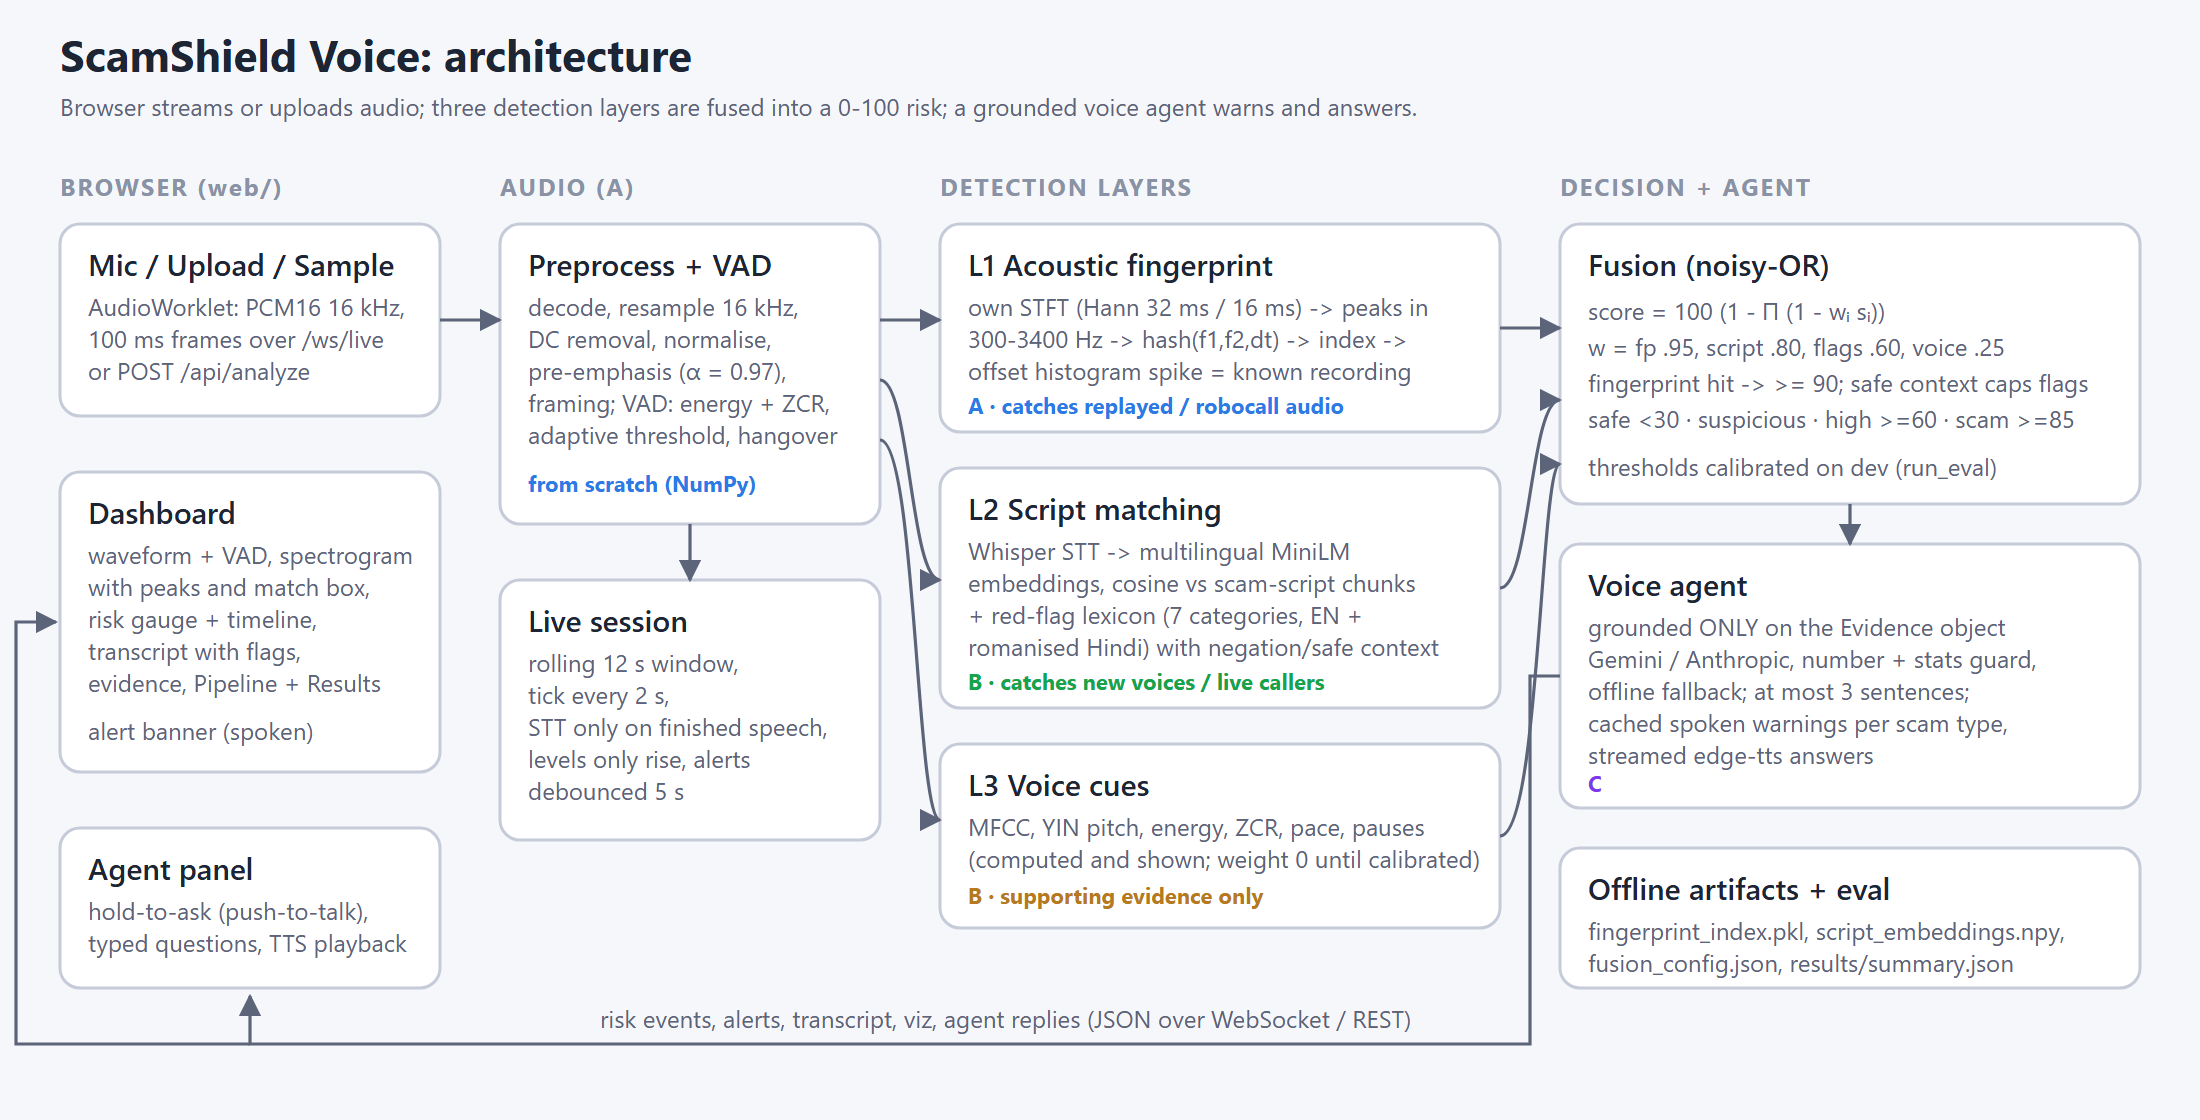
\includegraphics[width=\columnwidth]{Figures/fig_architecture.png}
\caption{\label{fig:arch}Architecture of ScamShield Voice. Layer 1 (acoustic fingerprint) catches replayed recordings, Layer 2 (speech-to-text, wording model and red-flag lexicon) catches new voices and live callers, Layer 3 (voice cues) is supporting evidence, and the fusion output grounds the voice assistant.}
\end{figure}

\subsubsection{Data}
\paragraph{Library and phone-line variants.} We wrote 17 fictional scripts: 10 scams of six types (digital arrest, KYC/OTP, lottery prize, relative in trouble, fake courier, tech support) and 7 genuine calls (bank alert, OTP notice, delivery, appointment, friend, in English and romanised Hindi, ``Hinglish''). Each was synthesised with four neural voices at two speaking rates, giving 136 clean clips, and each clip was degraded in seven ways (telephone band-pass 300--3400~Hz with 8~kHz resampling, white noise at 20, 10 and 5~dB SNR (the 5~dB version is also telephone-filtered), a GSM~6.10 codec round trip, and speed changes of $\pm$5\%), giving 952 further clips. All names, numbers and amounts are fictional.

\paragraph{Generated corpus.} Scripts written by us alone are too few and too similar to each other to train a model, so we generated a corpus with a large language model (Gemini) under fixed prompts for each scam and genuine-call category, mixing tones, personas and languages. The \emph{train} set has 612 scripts (500 scam, 112 genuine), of which 152 were added after we found that prompts which told the generator to avoid keywords had taught the classifier that ``OTP'' means genuine (Section~\ref{sec:model}). A \emph{dev} set of 166 scripts was generated separately for calibration. A \emph{test~2} set of 160 scripts was generated by a \emph{different model with a differently worded prompt}, and its SHA-256 hash was recorded before any model was trained; the evaluation program refuses to run if the file has changed.

\paragraph{Evaluation splits.} Table~\ref{tab:splits} lists the splits. The dev and test splits use the library scripts read by different voices, the holdout is a set of 18 scripts we wrote by hand with different wording and details, and dev~2 and test~2 are generated-corpus scripts synthesised with voices that appear nowhere else and passed through the full pipeline (synthesis, speech recognition, model). Dev and test clips are evaluated in all eight versions; dev~2 and test~2 clips in two, clean and telephone-filtered.

\begin{table}[H]
\centering
\caption{Evaluation splits. Every clip goes through the real pipeline.}
\label{tab:splits}
\resizebox{\textwidth}{!}{\tabsplits}
\end{table}

\subsubsection{Preprocessing, framing and voice activity detection}
Audio is converted to mono, resampled to 16~kHz with a polyphase filter, the mean is removed and the peak normalised to 0.99. Pre-emphasis flattens the spectral tilt of voiced speech:
\begin{equation}
y[n] = x[n] - \alpha\, x[n-1], \qquad \alpha = 0.97 .
\end{equation}
The signal is cut into frames of 25~ms with a 10~ms hop. For each frame we compute the short-time energy and the zero-crossing rate
\begin{equation}
E_k = \sum_{n} x_k^2[n], \qquad Z_k = \frac{1}{2(N-1)}\sum_{n=1}^{N-1}\bigl|\operatorname{sgn}(x_k[n]) - \operatorname{sgn}(x_k[n-1])\bigr| .
\end{equation}
The voice activity detector adapts to each recording. Let $F$ be the 10th and $P$ the 95th percentile of the frame energies in dB, and $D = P-F$. A frame is speech if $E_k > F + 0.3D$, or if it is weaker but noisy, $E_k > F + 0.15D$ and $Z_k > 0.25$, which keeps unvoiced fricatives such as /s/ and /f/. Gaps shorter than 200~ms are bridged, segments shorter than 100~ms are dropped, and a recording with less than 10~dB between $F$ and $P$ is declared silent. Figure~\ref{fig:signal} shows the result on one recording.

\begin{figure}[H]
\centering 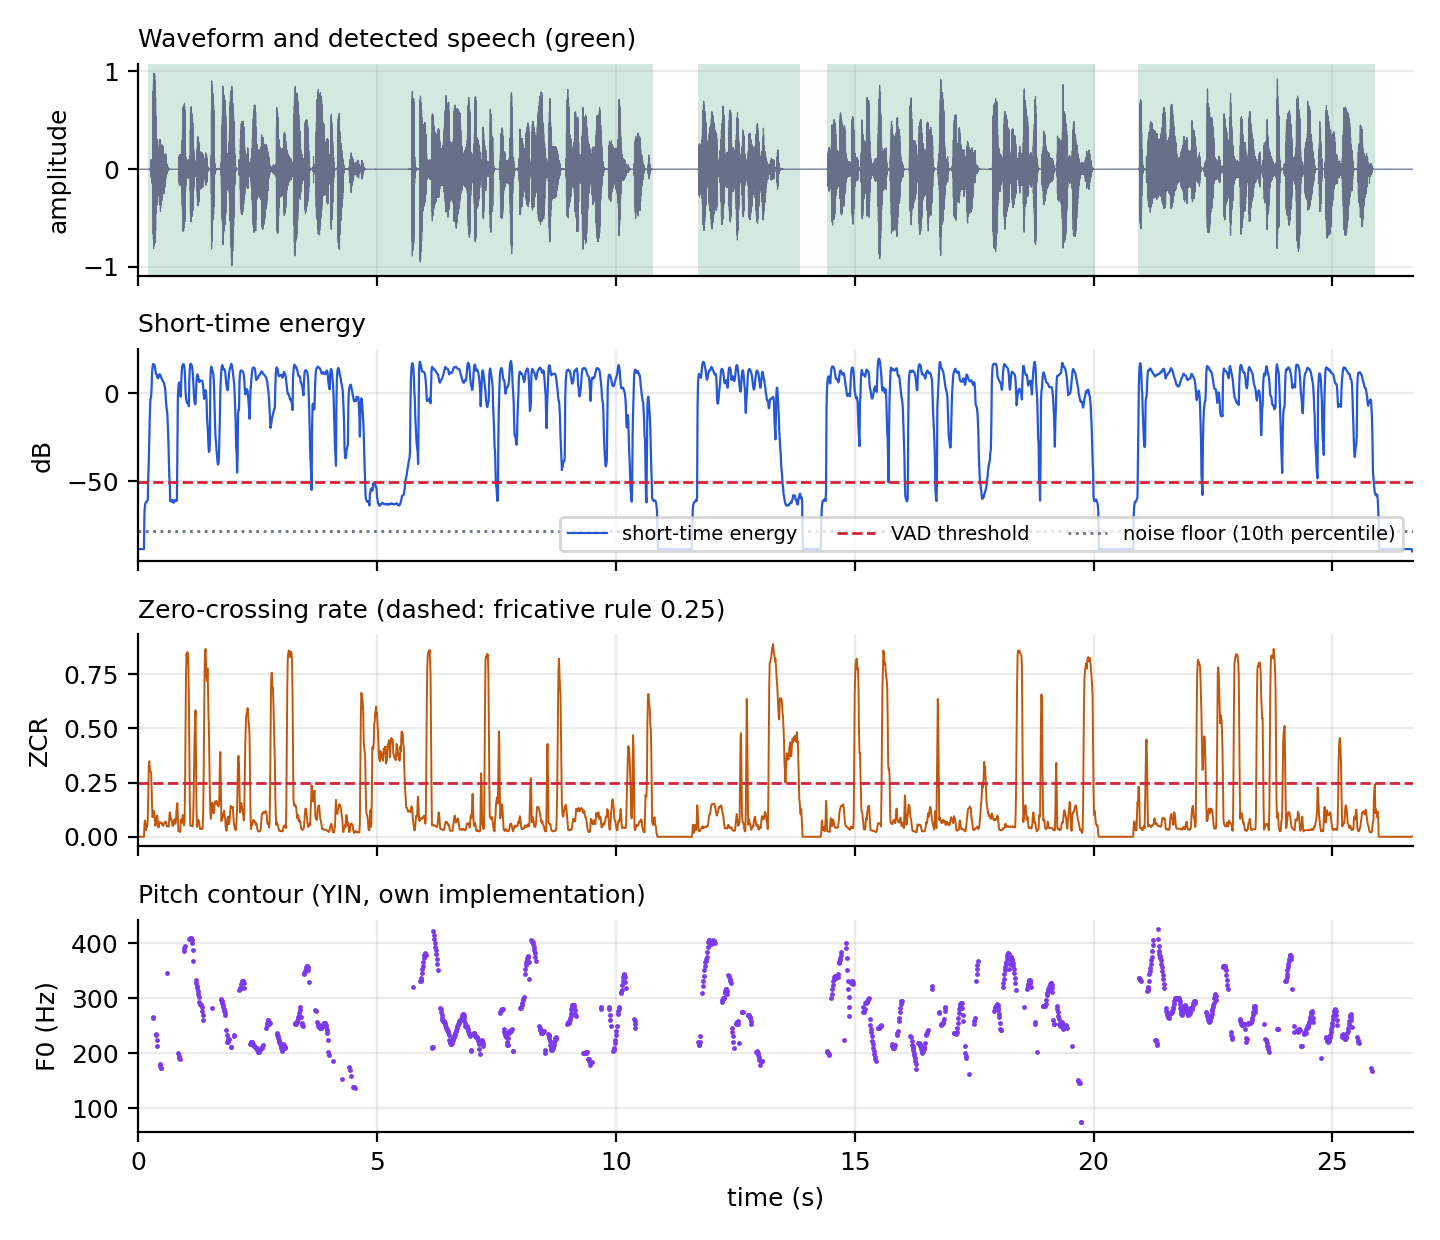
\includegraphics[width=0.92\columnwidth]{Figures/fig_signal.png}
\caption{\label{fig:signal}Time-domain analysis of a scam recording by our own code: detected speech regions, short-time energy with the adaptive threshold, zero-crossing rate with the fricative rule, and the YIN pitch contour.}
\end{figure}

\subsubsection{Spectrogram and spectral peaks}
The spectrogram is a short-time Fourier transform with a 512-point Hann window (32~ms) and a hop of 256 samples (16~ms),
\begin{equation}
X[k,m] = \sum_{n=0}^{N-1} x[n + mH]\, w[n]\, e^{-j 2\pi k n / N}, \qquad S_{\mathrm{dB}}[k,m] = 20\log_{10}\bigl(|X[k,m]| + \varepsilon\bigr),
\end{equation}
with $w[n] = 0.5 - 0.5\cos(2\pi n/N)$. A cell is a \emph{peak} if it is the maximum of its $15\times15$ (frequency $\times$ time) neighbourhood, lies in the band 300--3400~Hz, is more than 6~dB above the median of that band and within 60~dB of its maximum, and at most 30 peaks per second are kept. Restricting peaks to the telephone band lets a band-limited query share peaks with a full-band library clip. Neighbourhood maxima use the SciPy maximum filter; every other step is our own code.

\subsubsection{Hashing, index and matching}
Each anchor peak $(f_1, t_1)$ is paired with the next eight peaks $(f_2, t_2)$ whose time gap lies between 0.1 and 2.0~s. A pair becomes a 32-bit hash
\begin{equation}
h = (f_1 \ll 17)\ \mathrm{|}\ (f_2 \ll 8)\ \mathrm{|}\ \Delta t_q, \qquad \Delta t_q = \bigl\lfloor (t_2 - t_1)/\text{32 ms}\bigr\rfloor ,
\end{equation}
which encodes only \emph{relative} time, so it is the same wherever the clip starts. The index maps each hash to the library clips and anchor times where it occurs. For a query, every matching hash votes for the offset $t_{\text{library}} - t_{\text{query}}$ of each clip. If the query is an excerpt of a known recording, many hashes vote for \emph{one} offset and the histogram shows a spike; random collisions spread out (Figure~\ref{fig:fp}). The score of a clip is the number of aligned hashes, the largest vote count in a window of three adjacent offset bins, which tolerates $\pm1$ frame of jitter. The library holds one clip per scam script: 10 clips, 3\,640 peaks and 28\,628 hashes.

\begin{figure}[H]
\centering 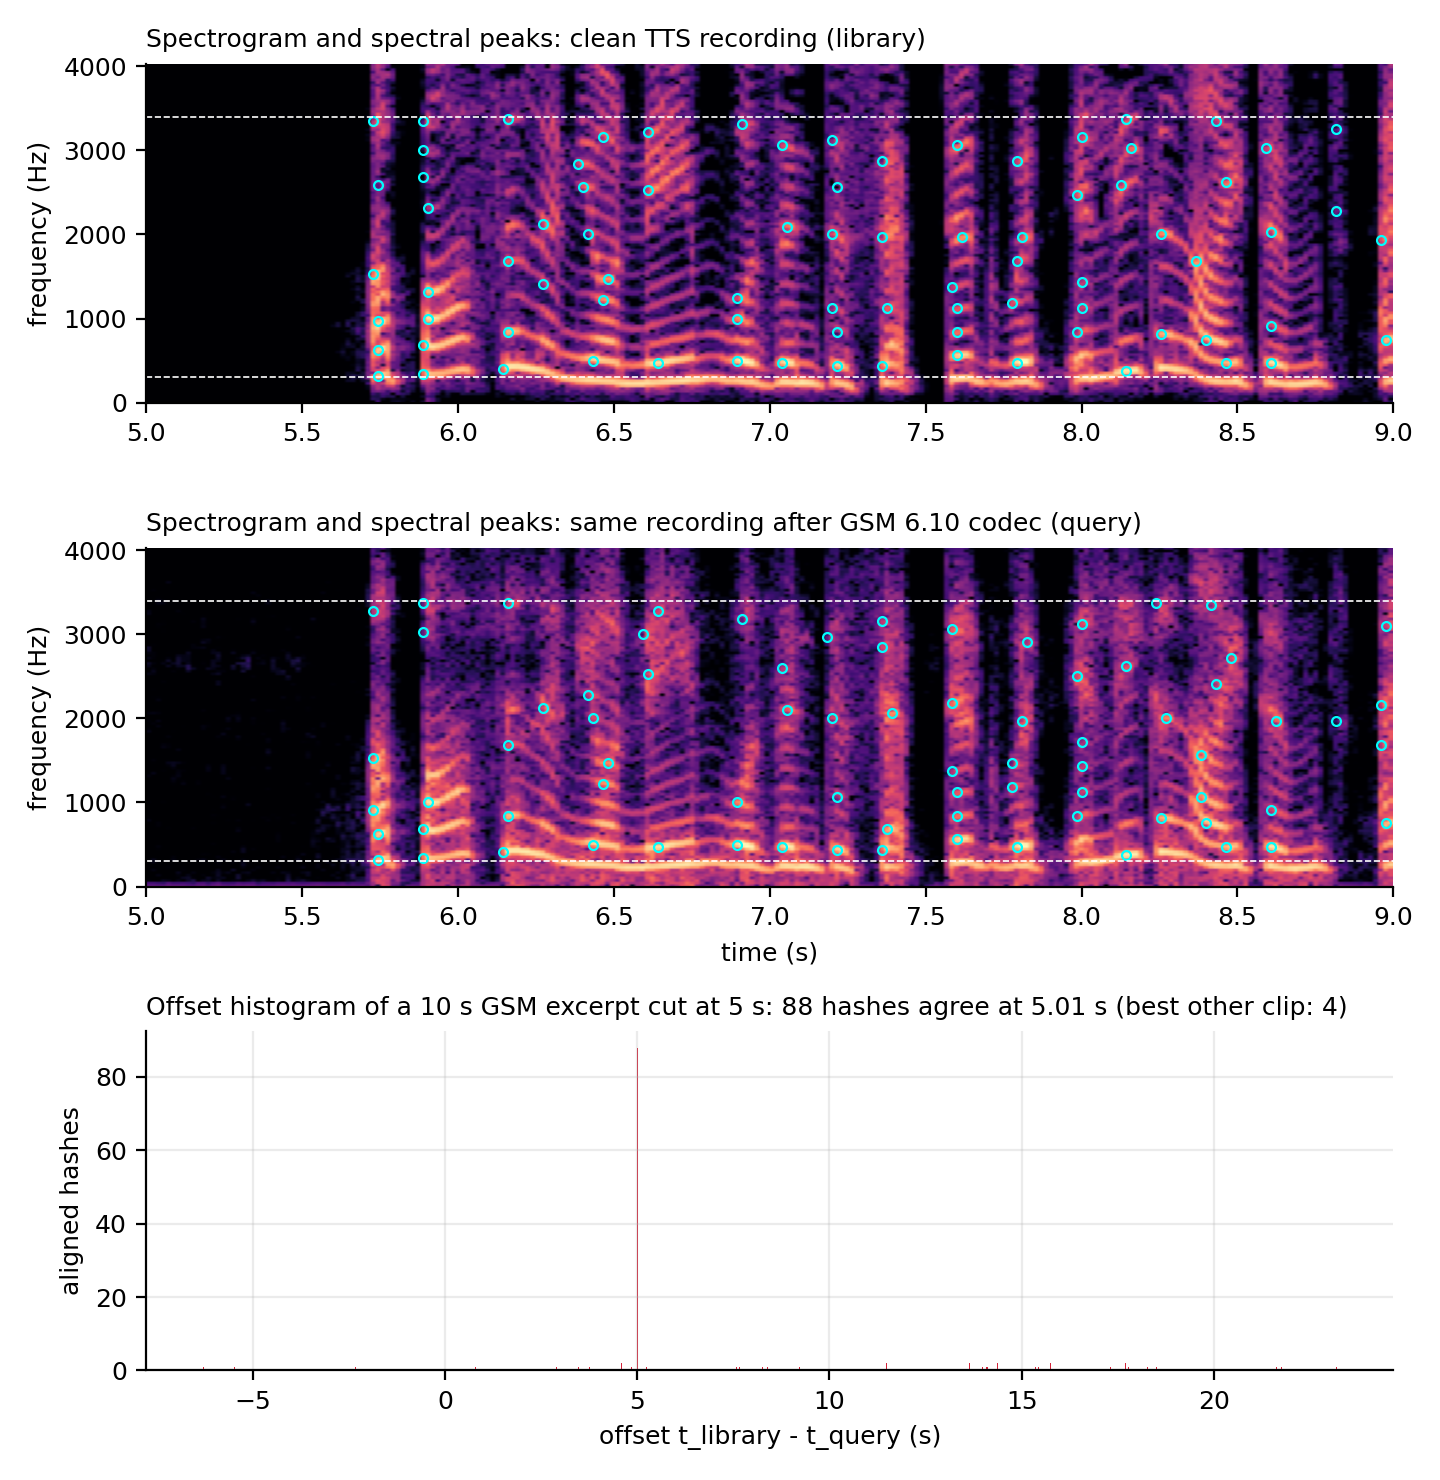
\includegraphics[width=0.9\columnwidth]{Figures/fig_fingerprint.png}
\caption{\label{fig:fp}Fingerprint of a scam recording. Top and middle: the same four seconds before and after a GSM codec, with the detected peaks (circles) and the telephone band (dashed). Many peaks survive the codec. Bottom: a 10~s excerpt of the degraded version cut at 5~s votes for the offset 5.01~s; the best wrong clip receives only 4 votes.}
\end{figure}

The decision threshold is calibrated on negatives: it is twice the largest number of aligned hashes obtained by any \emph{harmful} dev negative (genuine audio, or a match to the wrong script), plus one, which gave 25 aligned hashes (the worst negative scored 12). The match score reported to the fusion is $a/(a+25)$ for $a$ aligned hashes.

\subsubsection{MFCC and pitch}\label{sec:feat}
Mel-frequency cepstral coefficients are computed from Hamming-windowed 25~ms frames: the power spectrum of a 512-point FFT is passed through 26 triangular filters on the mel scale $m = 2595\log_{10}(1 + f/700)$, converted to decibels, and decorrelated by an orthonormal DCT-II, keeping 13 coefficients~\cite{davis1980mfcc}. Pitch is tracked with YIN~\cite{decheveigne2002yin}. For a 512-sample window the difference function
\begin{equation}
d(\tau) = \sum_{j=0}^{W-1}\bigl(x[j] - x[j+\tau]\bigr)^2
\end{equation}
is computed with the FFT, normalised by its cumulative mean, $d'(\tau) = d(\tau)\,\tau / \sum_{k\le\tau} d(k)$, the first lag with $d'(\tau) < 0.1$ is refined to a local minimum and a parabolic interpolation gives $f_0 = f_s/\tau$ (60--400~Hz). Pitch mean and standard deviation, the pause ratio from the voice activity detector, and the energy variation form the voice cues. They are shown to the user for context but carry no weight in the score, because we had no data to calibrate them.

\subsubsection{Speech recognition}
Speech is transcribed with Whisper~\cite{radford2023whisper} (the \texttt{base} model, 8-bit weights, on the CPU) through the \texttt{faster-whisper} library. Only the voice-activity segments are sent, grouped into chunks of at most 28~s cut at pauses, because Whisper invents text over silence~\cite{koenecke2024whisper}. We force English output: with automatic language detection, Hinglish was transcribed into Urdu or Devanagari script that our romanised patterns cannot read, whereas forced English output produces phonetic Latin text.

\subsubsection{The wording model}\label{sec:model}
The transcript is scored by a logistic regression on TF-IDF features~\cite{salton1988term}. The feature vector joins word 1--2-grams and word-bounded character 3--5-grams~\cite{cavnar1994ngram}, which make the model robust to the spelling variation of Hinglish and to small recognition errors:
\begin{equation}
d(\text{text}) = \mathbf{w}^{\top}\mathbf{x} + b, \qquad \mathbf{x} = \bigl[\ \mathrm{tfidf}_{\text{word}}\ \big|\ \mathrm{tfidf}_{\text{char}}\ \bigr].
\end{equation}
It is trained on the 612 generated training scripts. To choose it we compared designs on the generated dev set and on a \emph{shift probe}, the 17 hand-written scripts from our first dataset, which have a different author and were never used for training (Table~\ref{tab:select}). Matching a transcript to the closest of 10 known scripts, our first design, was close to chance on dev; adding genuine scripts as negatives helped most; the TF-IDF classifier separated both sets best. The first trained model had learned ``otp'' as a strong sign of a \emph{genuine} call (our generation prompt had told the generator not to repeat keywords), and a plain request to read out an OTP scored only $+0.87$. Adding 152 direct-wording scam scripts moved it to $+2.25$ while keeping the genuine OTP notice at $-2.20$.

\begin{table}[H]
\centering
\caption{Choosing the wording model (AUC; models trained on the generated train set only). The shift probe is the 17 hand-written scripts; ``--'' means those scripts were the library itself.}
\label{tab:select}
\begin{tabular}{@{}lrr@{}}
\toprule
Design & Generated dev & Shift probe \\ \midrule
Cosine to the 10 original scripts (first design) & 0.545 & -- \\
Cosine to 500 generated scam scripts & 0.701 & -- \\
Scam minus genuine similarity (top-5 mean) & 0.963 & 0.943 \\
Logistic regression on MiniLM sentence embeddings & 0.967 & 0.943 \\
Keyword lexicon (red flags) & 0.653 & -- \\
\textbf{TF-IDF word + character n-grams, logistic regression} & \textbf{1.000} & \textbf{1.000} \\
\bottomrule
\end{tabular}
\end{table}

For the user-facing evidence, a sentence-embedding model (a multilingual MiniLM~\cite{reimers2020multilingual}) retrieves the closest known scam script from 1\,252 chunks of 517 scripts.

\subsubsection{Red flags, safe context and fusion}
A small lexicon flags seven categories of scam wording (urgency, authority, secrecy, credential request, payment, threat, remote access) in English and romanised Hindi. A negation word in the seven words before a credential, payment or remote-access phrase marks the flag \emph{negated}, and phrases typical of genuine messages (``if this was not you'', ``we will never ask'') halve the weight of the remaining credential and payment flags, so that a genuine bank alert that says ``never share your OTP'' is not penalised.

The layers are fused with a noisy-OR, in which each layer is an independent chance that the call is a scam:
\begin{equation}
\text{score} = 100\Bigl(1 - \prod_{i}\bigl(1 - w_i s_i\bigr)\Bigr), \quad w = \{\text{fingerprint } 0.95,\ \text{wording } 0.80,\ \text{red flags } 0.60,\ \text{voice } 0.25\},
\end{equation}
where $s_i\in[0,1]$. A fingerprint match above its threshold forces the score to at least 90. The wording component maps the model's decision value linearly,
\begin{equation}
s_{\text{wording}} = \operatorname{clip}\!\Bigl(\frac{d - d_{lo}}{d_{hi} - d_{lo}},\,0,\,1\Bigr),
\end{equation}
with $d_{lo} = 0.737$, the 95th percentile of the decision values of genuine dev~2 calls, and $d_{hi} = 2.57$, the 25th percentile of the scam values; both were fitted on dev~2 through the full pipeline, so that speech-recognition errors are included. Scores below 30 are \emph{safe}, 30--60 \emph{suspicious}, 60--85 \emph{high} and 85 and above \emph{scam}; a call is ``flagged'' when it reaches high or scam. The weights are fixed, documented values, not fitted. Each component that contributes also produces a plain-language reason (for example, ``the wording is typical of a KYC / OTP scam''), used verbatim by the interface and the assistant.

\subsubsection{Live analysis}
In live mode the browser sends 16-bit, 16~kHz frames of 100~ms over a WebSocket. The server keeps the audio and, for every 2~s of audio, (i) fingerprints the last 12~s, remembering a match for the rest of the call; (ii) runs the voice activity detector and transcribes only speech that has ended (0.5~s of silence follows it, or 10~s of unbroken speech); (iii) rescores the wording and flags over the transcript so far; and (iv) updates a level tracker. The tracker lets the level \emph{rise} immediately but lowers it by one step only after the score has stayed below the level's lower bound for 10~s, and sends an alert when the level reaches high or scam, at most once every 5~s. A ``simulated live'' mode streams a file through the same path at real-time speed, which is how we evaluate live behaviour reproducibly.

\subsubsection{Voice assistant and implementation}
The assistant receives an \emph{evidence object} (score, level, reasons, closest scripts, flagged phrases and the end of the transcript) and the user's question. Its prompt allows four things: facts about this call, only from the evidence; a short description of itself and what it can do; one-sentence replies to greetings and thanks; and a friendly redirect for unrelated topics. Replies are limited to three sentences, and a guard rejects any reply containing a number that is not in the evidence, or a statistic word, in which case a template answer built from the evidence is used; the same template serves when no language-model key or network is available. Spoken warnings for each scam type are pre-generated with a text-to-speech library and cached, so a warning starts immediately. Push-to-talk uses the browser's recorder and the speech recogniser. While the assistant speaks the microphone is muted, and the simulated call pauses, so the two never overlap.

The back end is Python with FastAPI; the front end is plain HTML, JavaScript and canvas drawing without a build step, with light and dark themes. The code is public at \url{https://github.com/chrisxcalvin/Scam-call-fingerprinting}. A single command (\texttt{python scripts/run\_demo.py}) checks the setup, builds the library and starts the application; 60 automated tests cover the signal processing, the models, the web API and the live pipeline.

\section{Results and Discussion}\label{sec:results}
\subsection{Validation of the signal processing}
Libraries are used only for checking, never inside the system. Table~\ref{tab:dsp} compares our code with SciPy and librosa~\cite{mcfee2015librosa} on six real clips of our dataset. Our STFT matches SciPy's to better than $2.4\times10^{-6}$~dB and our mel filterbank matches librosa's to $3\times10^{-8}$. Our MFCCs match librosa's with a median absolute difference of about $10^{-7}$ and a minimum per-coefficient correlation of 0.9988 or better. Two conventions had to be aligned for this comparison: librosa centres the 400-sample window inside its 512-sample FFT frame, a 56-sample shift, and its default Hamming window is periodic whereas ours is symmetric. Before alignment our first comparison gave correlations of only 0.95--0.98, which showed the check was sensitive. The remaining larger differences (up to 4.5 on values of several hundred) occur only in near-silent frames, where our additive $10^{-10}$ floor and librosa's clipping floor differ. Our YIN tracker agrees with librosa's within 5\% on 97--99\% of voiced frames for five clips; for the sixth, a bank-alert voice, agreement is only 60\%, although both trackers report the same median pitch (181~Hz), so it is not an octave problem and we did not find the cause.

\begin{table}[H]
\centering
\caption{Our DSP code against reference libraries on six synthetic-speech clips (C1--C6). STFT against SciPy; MFCC against librosa (aligned, symmetric window); F0 against \texttt{librosa.yin} on the frames our tracker calls voiced.}
\label{tab:dsp}
\resizebox{\textwidth}{!}{\tabdsp}
\end{table}

\subsection{Fingerprint under degradation}
Table~\ref{tab:fp} and Figure~\ref{fig:aligned} report the exact library recordings after each degradation, pooled over the dev and test splits (10 queries per condition). Every query was identified correctly in every condition, and none fell below the threshold. Evidence is strongest for the clean and telephone-band versions (about 2\,200--2\,500 aligned hashes), drops to roughly 600--1\,000 under the GSM codec and noise, and falls to a median of 83--104 for a speed change of $\pm$5\%, because a speed change shifts every frequency and time difference. Even the weakest query (62 hashes) is 2.5 times the decision threshold of 25 and five times the worst negative (12). Across all five splits no legitimate or unrelated clip was matched (0 of 1\,459 harmful negatives). Same-script audio in the library voice at the other speaking rate is a near-copy of the indexed recording; it matched its own script in 22--28\% of cases, which we report separately because it is not a false match. A query over a full clip takes about 20~ms (median).

\begin{table}[H]
\centering
\caption{Fingerprint identification of the exact library recordings (dev and test pooled).}
\label{tab:fp}
\resizebox{0.9\textwidth}{!}{\tabfp}
\end{table}

\begin{figure}[H]
\centering 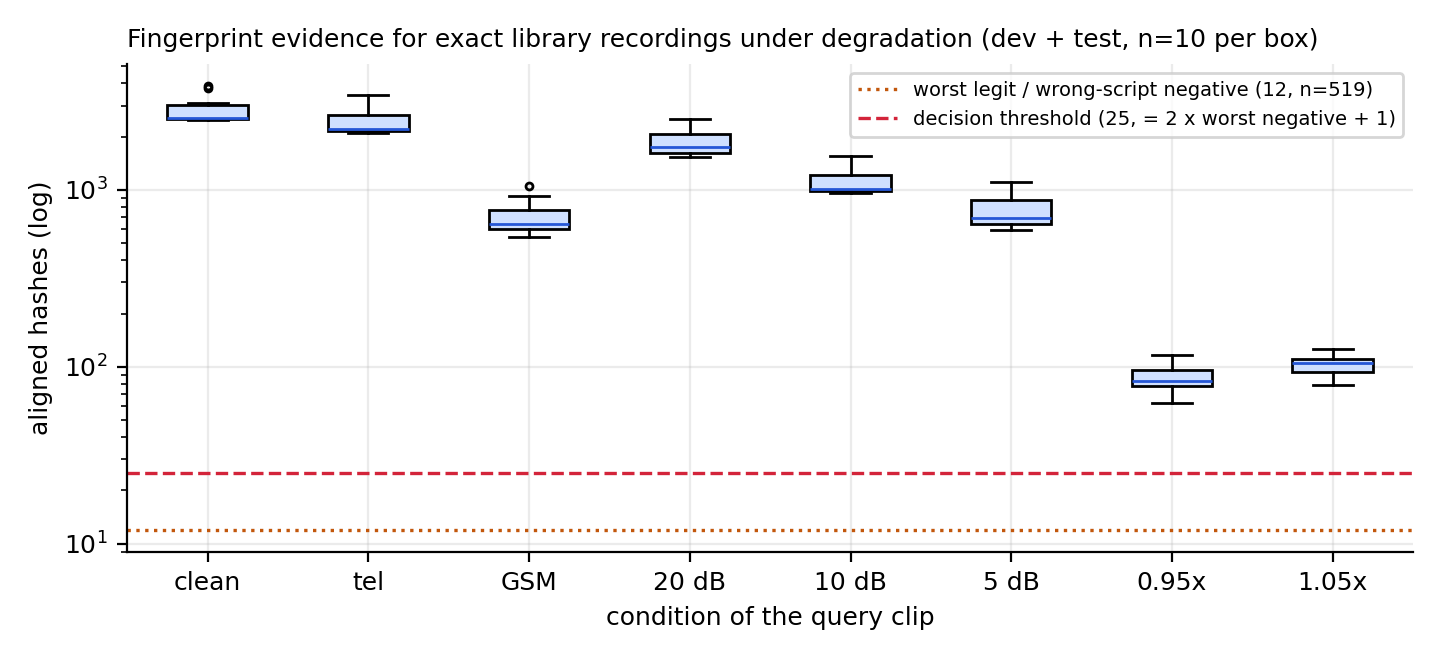
\includegraphics[width=0.9\columnwidth]{Figures/fig_aligned.png}
\caption{\label{fig:aligned}Aligned hashes for exact library recordings under each degradation (log scale), with the worst negative and the decision threshold.}
\end{figure}

\subsection{Detecting scams end to end}
Table~\ref{tab:main} gives the main result, and Figure~\ref{fig:roc} compares the scores. The numbers come from the full pipeline: synthesis, a telephone-band version, speech recognition, the wording model, the red-flag lexicon and fusion, and a clip counts as ``flagged'' at level high or scam.

\begin{table}[H]
\centering
\caption{Scam detection on unseen data (upload path). ``AUC (en / hi)'' is the area under the ROC curve~\cite{fawcett2006roc} of the wording model for English and Hinglish clips.}
\label{tab:main}
\resizebox{\textwidth}{!}{\tabmain}
\end{table}

\begin{figure}[H]
\centering 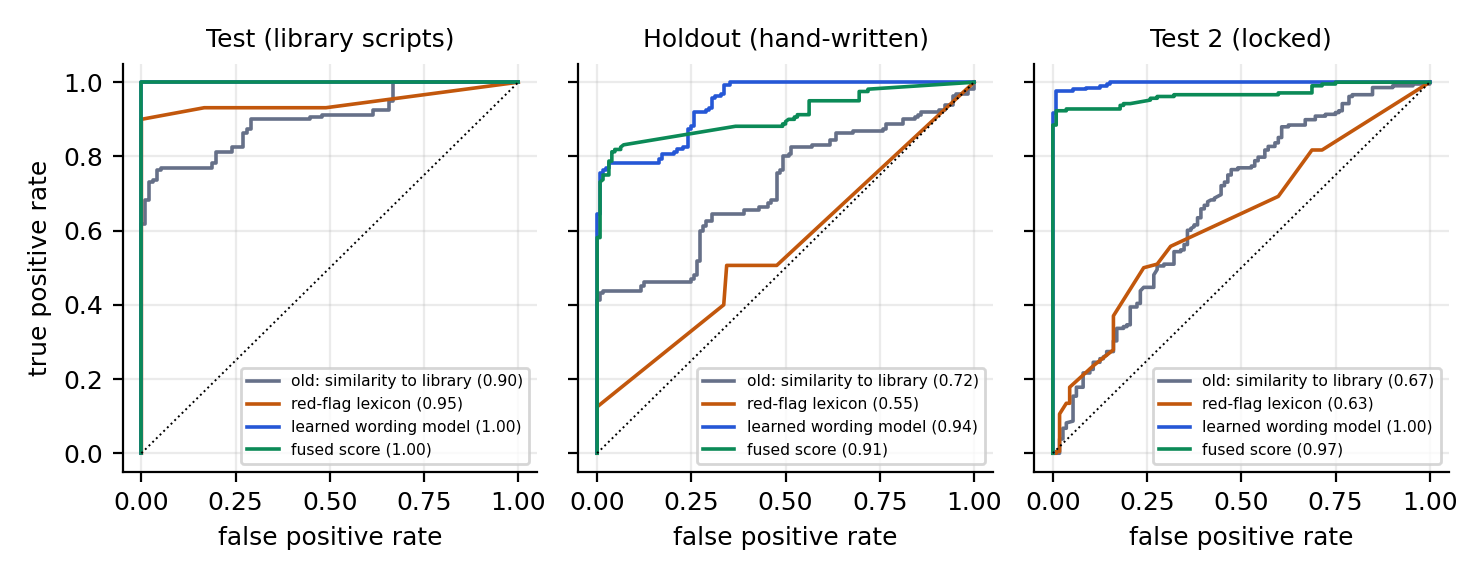
\includegraphics[width=\columnwidth]{Figures/fig_roc.png}
\caption{\label{fig:roc}ROC curves (area in brackets) for the old similarity-to-library score, the red-flag lexicon, the learned wording model and the fused score, on the old test split, the hand-written holdout and the locked test~2.}
\end{figure}

\paragraph{Locked test 2.} The system caught 92.3\% of scam clips (192 of 208) with 1.8\% false alarms (2 of 112 genuine clips) and a precision of 0.99. The wording model alone separates scam from genuine wording almost perfectly (AUC 0.997; 0.998 for English and 0.993 for Hinglish), even though test~2 was written by a different generator model, with a different prompt, read by unseen voices and passed through speech recognition (word error rate about 10\% on the English clips).

\paragraph{From 11\% to 73\% on the holdout.} The most instructive result is the hand-written holdout. With our first design (similarity to 10 known scripts plus the lexicon), only 18 of its 160 scam clips (11\%) were caught, whereas the old test split, which reuses the library scripts, had given 87.5\% with 6.2\% false alarms (both measured on the first version, before the learned model). The first design memorised its library. With the learned model, trained only on generated data, the same holdout reaches 73\% with one false alarm, and the old test split reaches 98.8\% with none. All six English reworded scams are now caught in every voice. The holdout's scripts were read while we diagnosed the first failure, so we treat it as a second look and not as a blind test; the blind result is test~2.

\paragraph{By scam type.} Figure~\ref{fig:type} shows the share of flagged clips on test~2 by type and language. Digital arrest, lottery and tech support are always flagged; KYC/OTP is the weakest (75\% in English and 62\% in Hinglish). Scam-type identification (which type was it?) is correct for 75\% of the scam clips.

\begin{figure}[H]
\centering 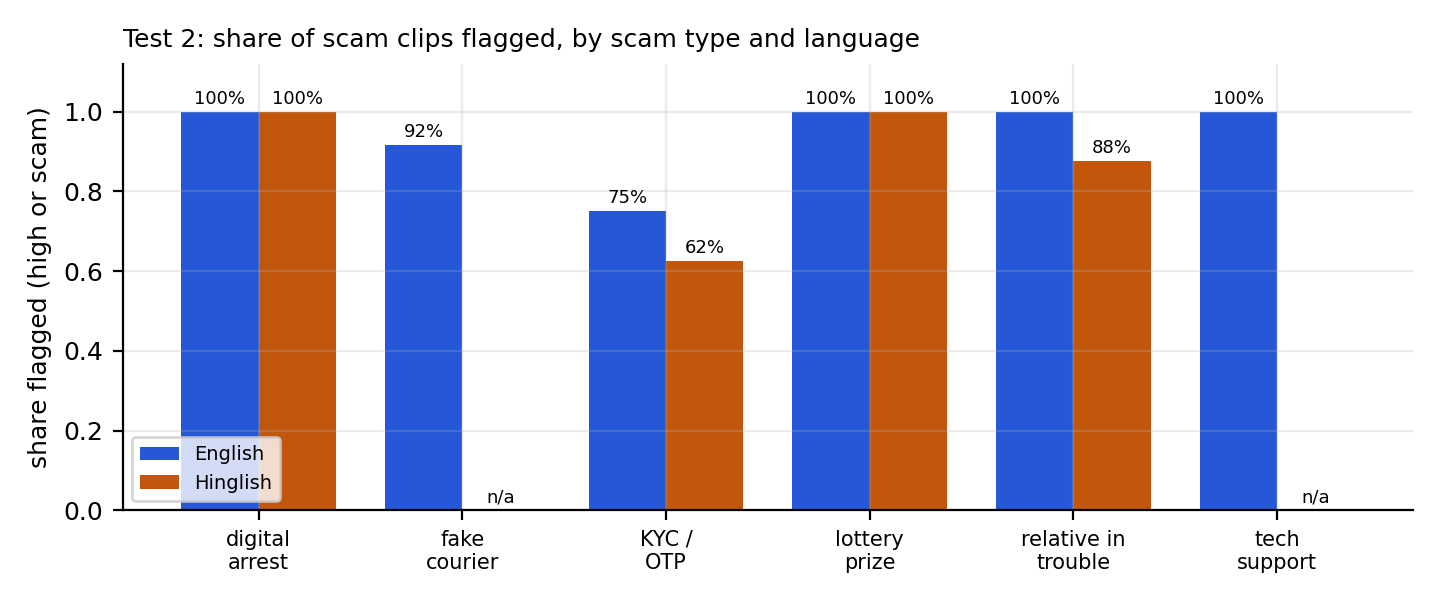
\includegraphics[width=0.92\columnwidth]{Figures/fig_by_type.png}
\caption{\label{fig:type}Test~2: share of scam clips flagged (high or scam), by scam type and language (``n/a'': no scripts of that type in Hinglish).}
\end{figure}

\paragraph{Hinglish.} Hinglish is the hardest case. On the hand-written holdout, wording AUC is 0.69 for Hinglish against 1.00 for English, and Hinglish KYC/OTP and lottery calls are mostly missed, although on generated test~2 the Hinglish AUC is 0.993. Hinglish in the training corpus was written by the language model and differs in style from the Hinglish we wrote by hand, and speech recognition of Hinglish is poor (it often produces phonetic nonsense); we expect real callers to vary even more.

\subsection{What each layer contributes}
Table~\ref{tab:abl} shows the ablation on test~2. The fingerprint layer scores zero here by construction, because none of the clips is a recording from the library; its contribution is to replayed scams (previous subsection). The wording model alone catches 77\% of scam clips with no false alarm, and fusion raises this to 92\% at the cost of two false alarms. The red-flag lexicon is weak: its AUC is only 0.63 on test~2 and 0.55 on the holdout, because paraphrased scams avoid its keywords (``tell me that code'' instead of ``OTP'') while honest notices contain them, and fusing it in lowers the ranking quality compared with the wording model alone (fused AUC 0.967 against 0.997 on test~2). We kept the lexicon because it makes the reasons readable, but the evidence suggests down-weighting it.

\begin{table}[H]
\centering
\caption{Ablation on locked test~2 (flagged = high or scam).}
\label{tab:abl}
\resizebox{0.9\textwidth}{!}{\tabablation}
\end{table}

\subsection{Live detection and its main weakness}
Table~\ref{tab:live} reports the live simulation. Replayed scam recordings raise an alert after about 2~s, before the first scam phrase has finished, because the fingerprint of the first seconds already matches. Scams in new voices raise an alert a median of 4.5~s \emph{before} the end of the first sentence that contains a lexicon keyword on test~2, because the learned wording model reacts to earlier sentences than the keyword lexicon does; 91\% of them alert within 5~s of that sentence. About 97\% of scam streams alert at some point on test~2.

\begin{table}[H]
\centering
\caption{Live simulation. ``Latency'' is the time from the end of the first sentence containing a lexicon keyword to the first alert (negative: the alert came earlier).}
\label{tab:live}
\resizebox{\textwidth}{!}{\tablive}
\end{table}

The weakness is on the genuine side: 36\% of genuine test~2 streams (40 of 112) and 22\% of holdout streams reached the alert level at some point, against 1.8\% and 0.8\% on the upload path, and none on the old test split. Figure~\ref{fig:live} shows why for a genuine hospital call. Its first sentences (``your son had a minor fall'') resemble a relative-in-trouble scam; the score crosses the alert line at 8~s, and by the end of the call, when the reassurance has been said, it falls back below the flag line, yet the alert has been sent and the level cannot fall quickly. The upload path sees the whole call and does not have this problem. Fixing it, for example by requiring the evidence to persist over several checks or by letting contradicting evidence lower the level, is the main open improvement; because it was designed after seeing this result it would need new data for a clean test.

\begin{figure}[H]
\centering 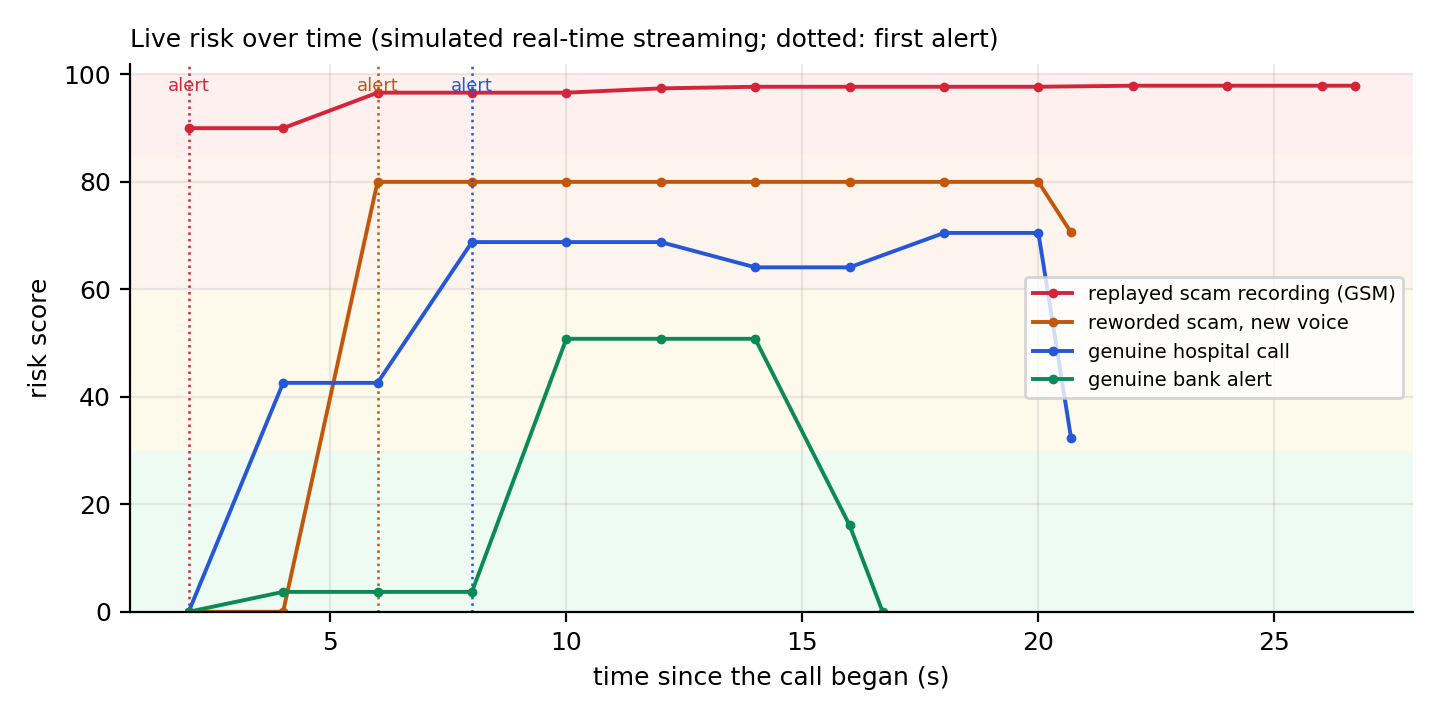
\includegraphics[width=0.92\columnwidth]{Figures/fig_live.png}
\caption{\label{fig:live}Live risk over time for four calls. The replay alerts at 2~s. The reworded scam alerts at 6~s. The genuine hospital call opens like a scam, alerts at 8~s and then falls back, which the level tracker does not follow in time.}
\end{figure}

\subsection{Speed}
Table~\ref{tab:lat} lists the time per stage for a typical clip of about 20~s on a laptop CPU (median over the old test split; speech recognition time is that of the first uncached run). The signal-processing stages together take well under a quarter of a second; Whisper dominates. In live mode one analysis step takes a median of 25--37~ms apart from the occasional speech-recognition call.

\begin{table}[H]
\centering
\caption{Time per stage for the upload path (milliseconds).}
\label{tab:lat}
\resizebox{0.8\textwidth}{!}{\tablatency}
\end{table}

\subsection{The interface and the assistant}
Figure~\ref{fig:ui} shows the interface. The verdict (ring, plain-language title, reasons and a ``what to do now'' panel for risky calls) comes first; the four evidence tiles, the risk timeline, the transcript with marked phrases and the audio view follow, and the assistant sits beside them. In a 10-turn test conversation against the real language model, the assistant answered ``What are you?'' with a short description of itself, declined the weather question in one friendly sentence, gave different answers to the same question asked twice, and answered ``Should I give him the OTP? He sounds real'' with a clear ``no'', all without inventing a number. Before we rewrote its prompt, it had answered ``What are you?'' and ``Okay, thank you. Bye-bye'' with the same scam warning, because it was confined to the call evidence.

\begin{figure}[!t]
\centering
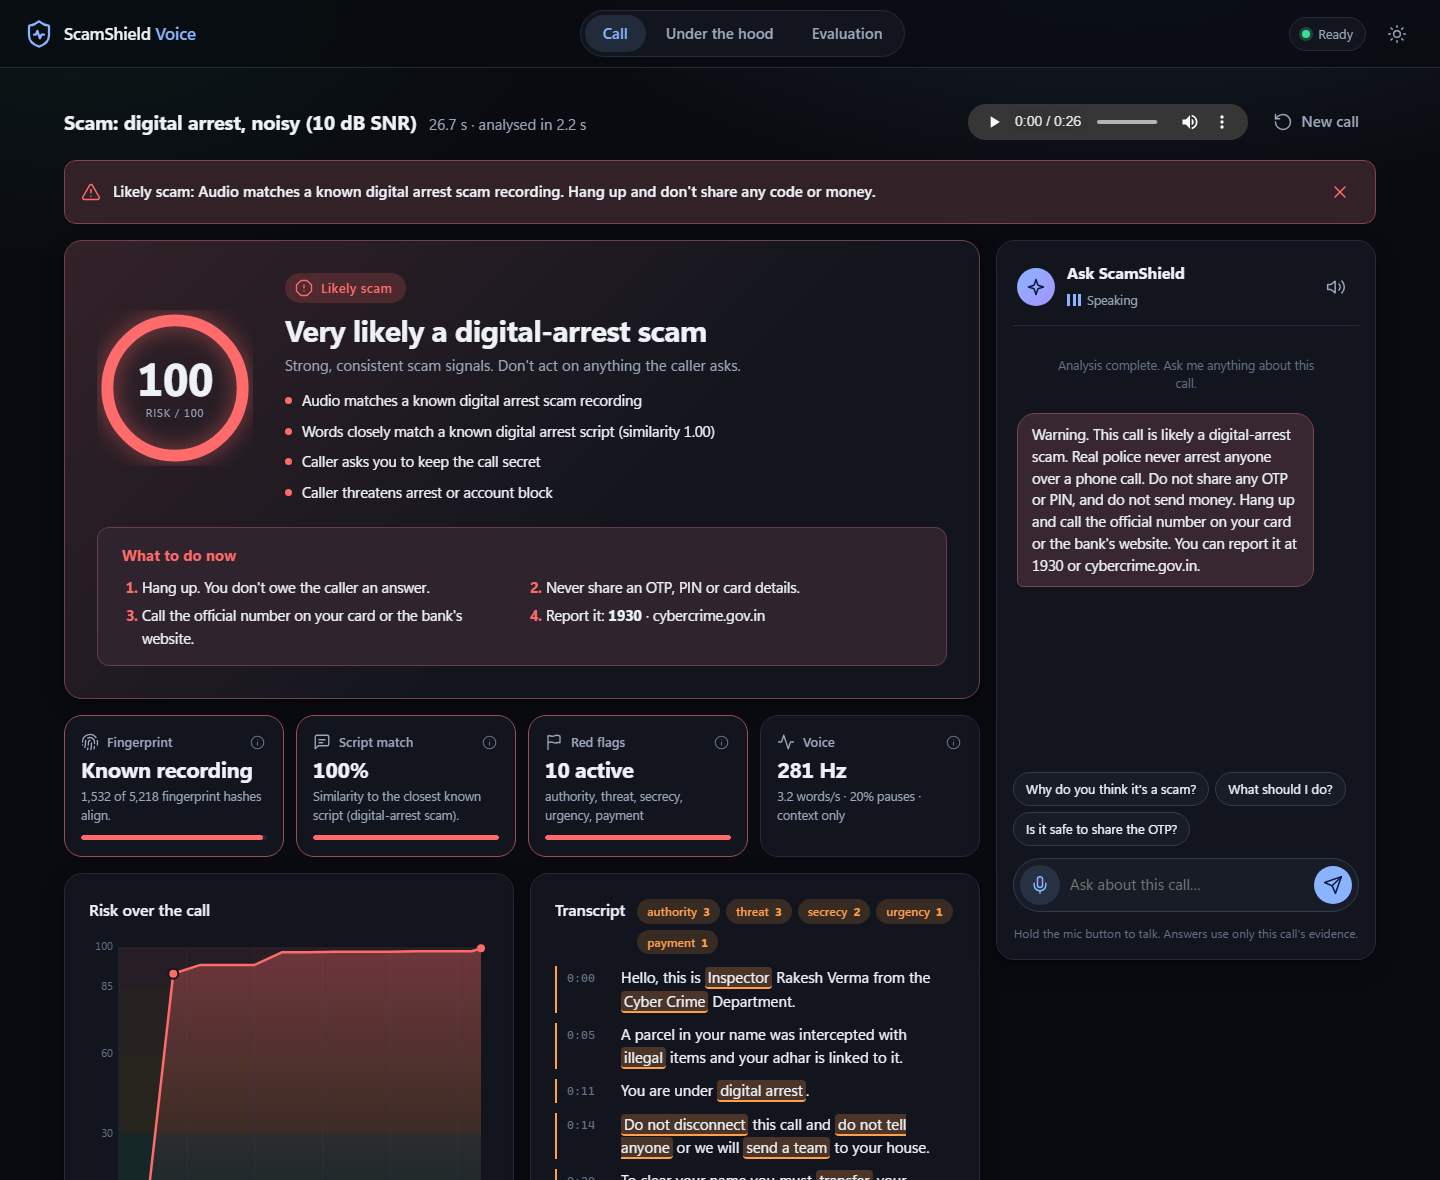
\includegraphics[width=0.66\columnwidth]{Figures/fig_ui_scam.png}\\[6pt]
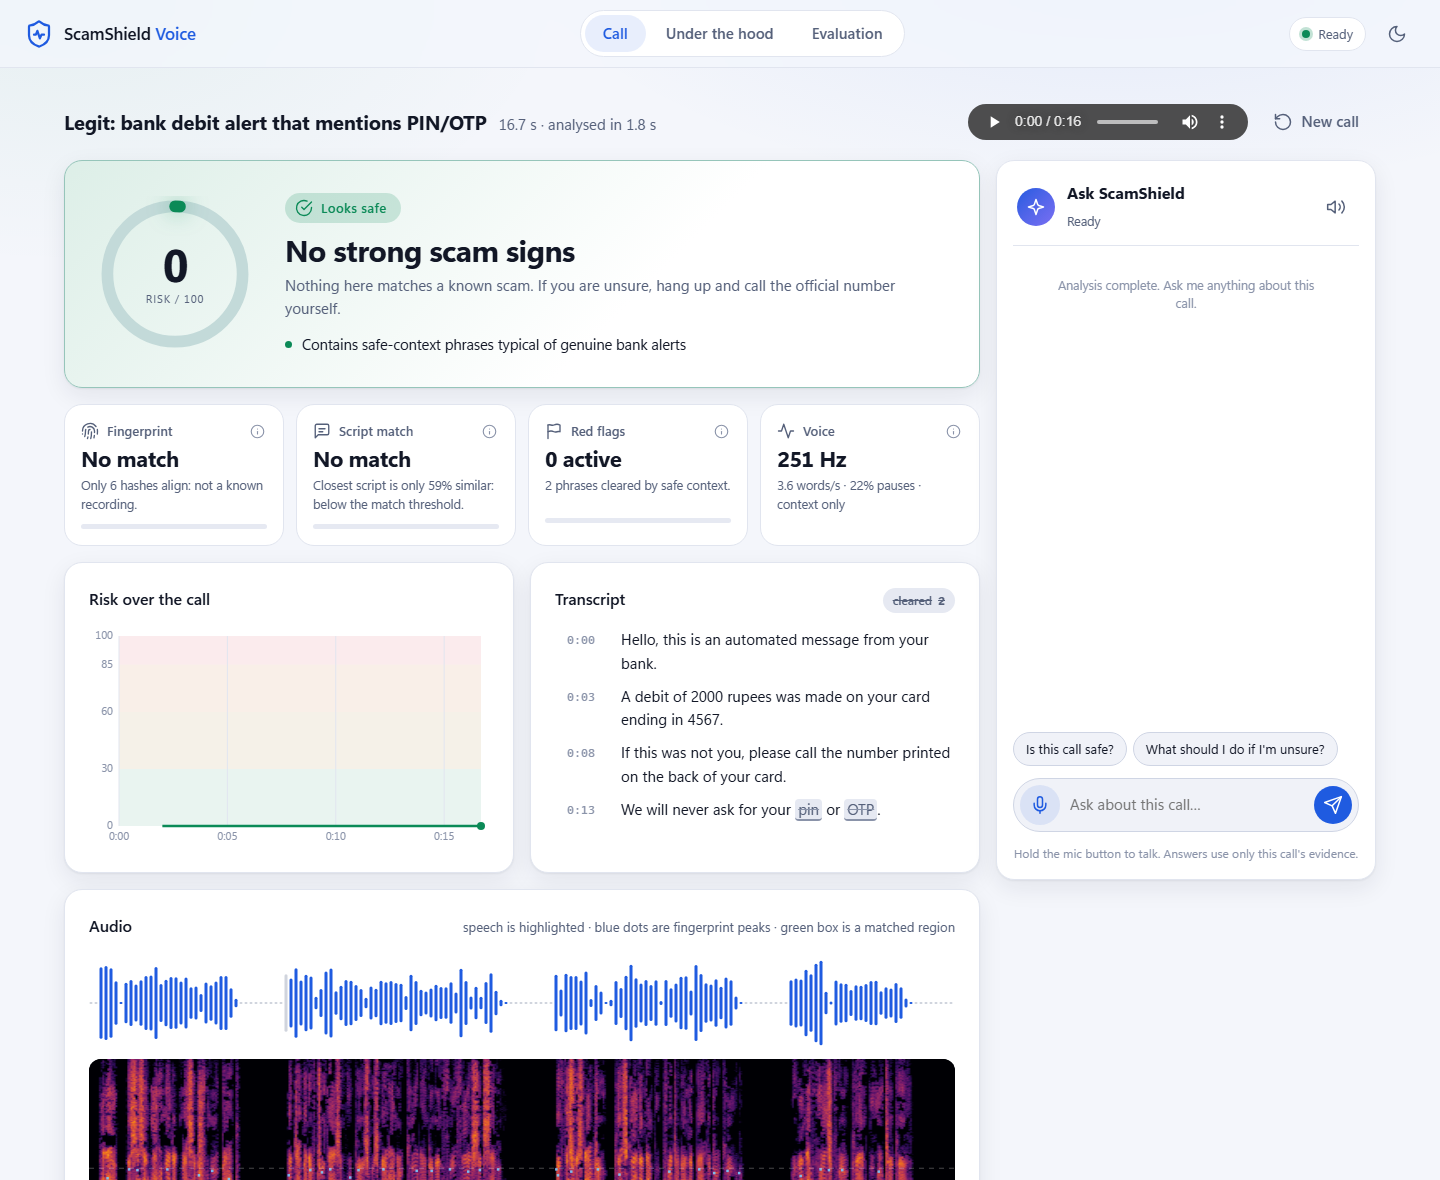
\includegraphics[width=0.66\columnwidth]{Figures/fig_ui_safe.png}
\caption{\label{fig:ui}Interface. Top: a scam call flagged by the fingerprint and the wording, with the verdict, a ``what to do now'' panel, the evidence tiles, the risk timeline, the transcript with marked phrases and the voice assistant (dark theme). Bottom: a genuine bank alert that stays safe because ``never share your PIN or OTP'' is recognised as safe context (light theme).}
\end{figure}

\subsection{Limitations}
\begin{itemize}
    \item \textbf{Synthetic speech.} All audio is neural text-to-speech with phone-line effects. Real human speech, accents, overlapping talk and genuine phone noise are untested, and we have no consented human recordings yet.
    \item \textbf{Generated text.} The wording model is trained on scripts written by a language model; real scammers will say things it has not seen. Test~2 shows it generalises to a different generator, not to real calls.
    \item \textbf{Live false alerts} on about a third of genuine calls in simulation (above).
    \item \textbf{Weakest cases:} KYC/OTP scams, and Hinglish (recognition by Whisper is poor and our Hinglish test data are few).
    \item \textbf{Known scams only.} The fingerprint recognises recordings already in the library; the wording model recognises scripts like those it has seen.
    \item \textbf{Deployment.} Phone operating systems do not give applications access to call audio, so the demonstration uses a microphone, a speakerphone or uploaded audio; analysing real calls also requires consent under privacy law. Audio is kept in memory only. We deliberately use stock voices and do not clone any real person's voice.
\end{itemize}

\section{Conclusions}\label{sec:conc}
ScamShield Voice shows that the signal-processing methods of this course are enough to build a useful scam-call detector, and that a small learned model fills the gap that fingerprints cannot cover. Our own fingerprint identified every known recording through a telephone filter, a GSM codec, noise and speed change with no false matches, and our DSP code matched SciPy and librosa. A learned wording model, trained on generated scripts and tested on a locked set from a different generator, caught 92.3\% of scam clips with 1.8\% false alarms.

The most valuable result was a failure. Our first Layer-2 design looked excellent on scripts it had seen and caught only 11\% of reworded scams on a hand-written holdout. Building that holdout, diagnosing the failure and replacing the design with a learned model trained on generated data raised the holdout to 73\% without ever training on it. A second finding is that streaming analysis acts on partial calls and raises false alerts on about a third of genuine calls in simulation, because some genuine calls open like scams.

In future work we would (i) let the live risk level fall when later evidence contradicts an early alert and require evidence to persist before alerting; (ii) collect consented human recordings, including Hinglish and real phone audio, and write a fresh independent test set; (iii) reduce the weight of the red-flag lexicon, which adds noise; (iv) add training data for KYC/OTP scams and for Hinglish; and (v) calibrate and use the voice cues.

%++++++++++++++++++++++++++++++++++++++++
\bibliographystyle{IEEEtran}
\bibliography{mybibliography}

\end{document}
